% !TeX program = xelatex
\documentclass[lang=cn,11pt,scheme=chinese,chinesefont=nofont,color=green]{elegantbook}

% ---------- 字体：与项目技术文档保持一致 ----------
\setCJKmainfont[Path=fonts/,
  BoldFont=FandolSong-Bold.otf,
  ItalicFont=FZKai.ttf,
  BoldItalicFont=FandolSong-Bold.otf
]{FZShuSong.ttf}
\setCJKsansfont[Path=fonts/]{FZHei.ttf}
\setCJKmonofont[Path=fonts/,Scale=0.94]{FZShuSong.ttf}
\setCJKfamilyfont{kaishu}[Path=fonts/,BoldFont=FandolSong-Bold.otf]{FZKai.ttf}
\setmainfont{Times New Roman}
\setsansfont{Noto Sans CJK SC}
\setmonofont{DejaVu Sans Mono}

\usepackage{amsmath,amssymb,bm}
\usepackage{graphicx}
\usepackage{booktabs}
\usepackage{array}
\usepackage{multirow}
\usepackage{makecell}
\usepackage{float}
\usepackage{caption}
\usepackage{xcolor}
\usepackage{listings}
\usepackage{enumitem}
\usepackage{url}

\captionsetup{font=small,labelfont=bf,labelsep=quad}
\setlength{\emergencystretch}{1em}
\AtBeginBibliography{\raggedright}
\setlist[itemize]{leftmargin=2em,itemsep=0pt,parsep=0pt,topsep=0.15em}
\setlist[enumerate]{leftmargin=2em,itemsep=0pt,parsep=0pt,topsep=0.15em}
\AtBeginDocument{%
  \setlength{\abovedisplayskip}{2pt plus 0pt minus 0pt}%
  \setlength{\belowdisplayskip}{2pt plus 0pt minus 0pt}%
  \setlength{\abovedisplayshortskip}{0pt plus 0pt minus 0pt}%
  \setlength{\belowdisplayshortskip}{0pt plus 0pt minus 0pt}%
}

\definecolor{deepgreen}{RGB}{18,59,50}
\definecolor{accent}{RGB}{47,125,104}
\definecolor{codebg}{RGB}{247,249,248}
\definecolor{codegray}{RGB}{110,110,110}
\definecolor{codeblue}{RGB}{30,70,140}
\definecolor{codegreen}{RGB}{30,110,80}
\definecolor{rulegray}{RGB}{180,190,186}
\colorlet{coverlinecolor}{accent}

\lstdefinestyle{proposalcode}{
  backgroundcolor=\color{codebg},
  basicstyle=\ttfamily\small,
  keywordstyle=\color{codeblue}\bfseries,
  stringstyle=\color{codegreen},
  commentstyle=\color{codegray}\upshape,
  breaklines=true,
  columns=fullflexible,
  keepspaces=true,
  frame=single,
  rulecolor=\color{rulegray},
  framesep=4pt,
  xleftmargin=0.5em,
  xrightmargin=0.5em,
  aboveskip=0.5em,
  belowskip=0.5em,
  showstringspaces=false
}
\lstset{style=proposalcode}

\hypersetup{
  pdftitle={面向绿色水务的 RISC-V 边缘多模态检漏终端方案书},
  pdfauthor={超级马里奥},
  pdfsubject={第三届 CIE RISC-V 大赛方案书}
}

\title{面向绿色水务的\\[0.2em]RISC-V 边缘多模态检漏终端}
\subtitle{第三届 CIE RISC-V 大赛方案书}
\author{超级马里奥}
\date{2026 年 11 月}
\version{1.0}
\extrainfo{项目源代码：\url{https://github.com/Lvshujun0918/AI_Water}}
\cover{figures/cover_proposal.pdf}

\addbibresource{reference-proposal.bib}

\begin{document}

\maketitle

\frontmatter

\chapter*{摘要}
\addcontentsline{toc}{chapter}{摘要}
\markboth{摘要}{摘要}

城市供水管网漏损是一个被低估的“水—能—碳”问题。漏掉的水在到达用户之前，已经经历了取水、处理、加压输送，漏损因此同时意味着水资源浪费、电力消耗和碳排放。世界银行估计全球城市供水系统每年物理漏损约 320 亿立方米\cite{worldbank}；中国 2022 年城市公共供水漏损率为 12.89\%，2023 年降至 10\% 以内，政策目标是在 2025 年力争控制在 9\% 以内\cite{mohurd}。

本方案以进迭时空 K1 为算力底座，设计一台面向阀井、泵房和二次供水节点的边缘智能终端。系统以麦克风阵列采集管网声学信号，用 ResNetSE 声学事件识别模型在本地判断高风险、低风险和无风险；以语音识别把现场口令转为结构化意图；以本地小参数大模型解释风险、生成工单并回答运维问题；所有结果写入本地碳账本，形成可审计的“漏点—水量—电耗—碳排”证据链。工程重点是建立一套可复现的 RISC-V 深度学习运行时：以 Bianbu 为基座，锁定进迭时空 wheel 源中的 PyTorch 2.8.0、torchvision 0.23.0、torchaudio 2.8.0，移除 yeaudio、librosa、scipy、numba 在推理主路径上的脆弱依赖，并用 Docker 与 CI 固化交付。

本方案给出系统架构、技术实现、优化策略、用户文档、部署说明、测试报告、开发计划、预期成果和应用价值。当前仓库已实现声学识别链路、Web 管理端、RISC-V 运行时与容器构建；AMD64 基线已完成，RISC-V 侧已用 QEMU 用户态模拟验证模型加载、推理和 \texttt{predict.py} 端到端输出。K1 板端时延、功耗、ASR/LLM 实测数据仍按测试协议补充，方案不把设计目标写成实测结果。

\vspace{0.6em}
\noindent\textbf{关键词：} RISC-V；K1；边缘人工智能；供水管网；声学检漏；多模态交互；绿碳

\tableofcontents

\mainmatter

% =====================================================================
\chapter{引言}
\label{ch:intro}

\section{背景与问题}

供水管网是城市基础设施中最庞大、最隐蔽的资产之一。管道埋在地下，泄漏初期的地表迹象通常滞后，等到路面塌陷或居民水压下降时，损失已经扩大。世界银行的研究给出的全球物理漏损量约为每年 320 亿立方米\cite{worldbank}。这同时是一笔能源与碳的成本：水在被漏掉之前，已经经历了取水、混凝、沉淀、过滤、消毒和泵送。国际能源署估计，全球水部门（含取水、处理、输配和污水收集处理）消耗的电力约占全球总用电量的 4\%\cite{iea}。减少漏损，等于同时减少取水、处理和泵送三个环节的能耗。

中国的情况同样紧迫。公开资料援引《2022 年城市建设统计年鉴》指出，2022 年全国城市供水 635.45 亿立方米，漏损水量 81.91 亿立方米，漏损率 12.89\%；政策目标是到 2025 年全国城市公共供水管网漏损率力争控制在 9\% 以内\cite{mohurd}。从 12.89\% 降到 9\%，对应的是数十亿立方米的年节水量。

现有检漏方法各有局限。人工听音依赖经验，夜间作业强度大；相关仪定位精度较高，但需要两处接触，操作复杂；压力/流量分区计量能发现区域异常，却难以定位微小泄漏；光纤、卫星和无人机覆盖范围大，但成本高，不适合室内泵房。云端音频分析模型能力强，但依赖网络、带宽和隐私合规，难以在阀井和地下泵房稳定工作。实际管网需要“分区计量发现异常、声学终端确认漏点、人工现场复核”的组合，本方案聚焦其中最适合边缘部署的一环。

\section{参赛定位与目标}

方案的设计目标如下：

\begin{itemize}
  \item 声学单窗推理 p95 不超过 300 ms，语音指令端到端不超过 1 s；
  \item 在无 GPU、仅 2 TOPS 的 K1 上完成本地推理，典型整机功耗不超过 15 W；
  \item ASR、LLM、规则引擎与 Web 服务共享一套 RISC-V 运行时，断电重启可恢复；
  \item 碳账本记录漏点流量、提前发现时间、供水综合电耗与电网排放因子，数字可追溯；
  \item 代码、模型、容器、测试脚本和文档可复现，评委能按文档重新跑通。
\end{itemize}

\section{设计原则}

本方案坚持三条原则。第一，离线优先：声学推理、规则判断和碳账本写入都在本地完成，网络只负责结果同步与远程管理；断网时终端仍能告警和留痕。第二，证据优先：模型输出只是证据，动作由规则引擎和人工确认决定；每条工单绑定音频哈希、模型版本、置信度和操作员。第三，可复现优先：版本、wheel 源、ABI 路径、容器和测试脚本全部固定，评委可以在干净环境重建。

% =====================================================================
\chapter{技术实现}
\label{ch:tech}

\section{系统总体架构}

终端以 MUSE Pi Pro（K1，8 GB LPDDR4X，64 GB eMMC）为核心，按场景选配麦克风、4.3 英寸触摸屏、摄像头、WiFi/4G、eMMC/NVMe 和 40-pin GPIO。软件自下而上分为五层：硬件层、运行时层、智能层、服务层和交互层，如图\ref{fig:arch}所示。层间箭头表示调用与数据依赖，不表示所有进程均常驻。

\begin{figure}[htbp]
  \centering
  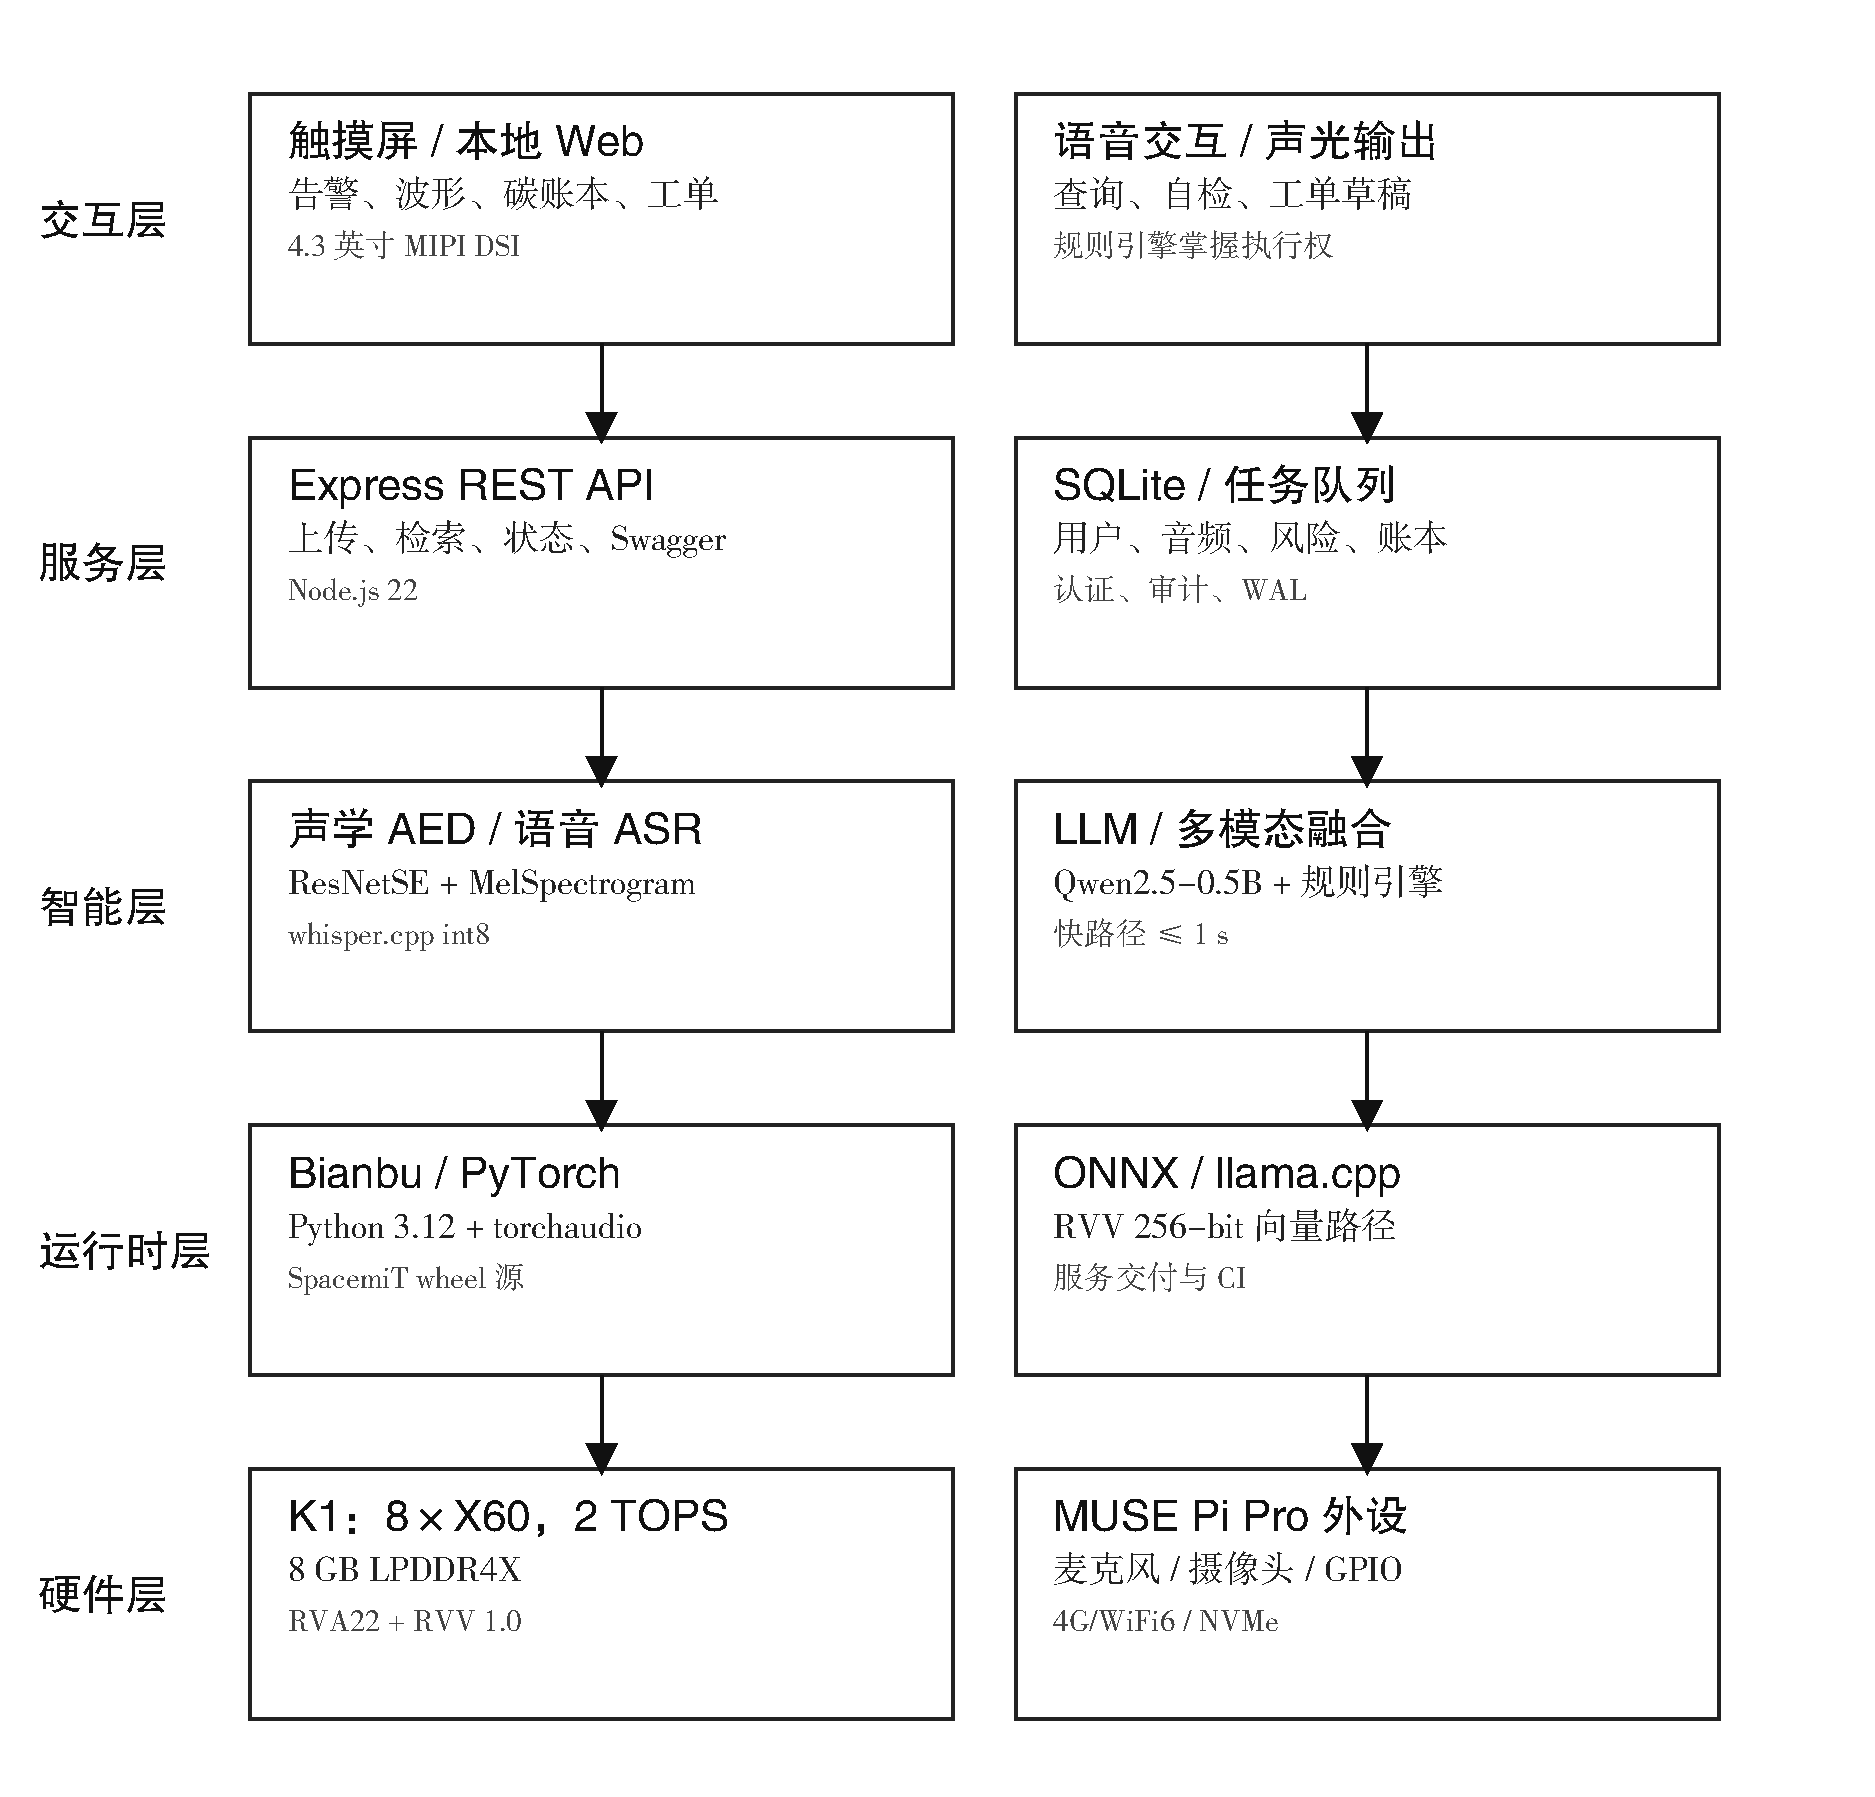
\includegraphics[width=0.90\linewidth]{figures/fig1_architecture.pdf}
  \caption{K1 边缘智能终端总体架构}
  \label{fig:arch}
\end{figure}

硬件层提供麦克风阵列、屏幕、摄像头、GPIO 与通信模组；运行时层是 Bianbu Linux、Python 3.12、Node.js 22、PyTorch 2.8.0 与 torchaudio 2.8.0；智能层包含声学事件识别、语音识别、本地 LLM 和多模态融合；服务层由 Express REST API、SQLite、任务队列、认证与审计组成；交互层提供本地 Web 管理端、触摸屏、语音与声光/继电器输出。

\begin{table}[htbp]
\centering
\small
\caption{边缘终端典型配置}
\label{tab:hardware}
\begin{tabular}{p{2.8cm}p{4.6cm}p{6.2cm}}
\toprule
部件 & 选型/接口 & 作用 \\
\midrule
主板 & MUSE Pi Pro，K1，8 GB & 本地推理、Web 服务、数据存储 \\
麦克风 & USB 阵列麦克风或模拟麦 + USB 声卡 & 采集 16 kHz 管网声音 \\
显示屏 & 4.3 英寸 MIPI DSI 触摸屏 & 现场告警、波形、工单确认 \\
摄像头 & OV5647，MIPI CSI（可选） & 高风险时拍照复核 \\
通信 & WiFi6 / 4G（miniPCIe） & 结构化结果回传 \\
存储 & eMMC + M.2 NVMe & 模型、音频证据、SQLite \\
执行 & 40-pin GPIO、继电器、蜂鸣器 & 声光告警与联动 \\
电源 & USB PD 3.0 & 单线供电 \\
\bottomrule
\end{tabular}
\end{table}

\section{声学检漏模型与数据}

声学检漏的基本原理是：高压水从破口喷出时形成湍流和空化，产生宽带噪声；声音沿管壁、土壤和空气传播，在阀门、消火栓、检查井等接触点可以被麦克风拾取。泄漏声的主要能量通常在几十赫兹到几千赫兹之间，具体频段受管材、管径、埋深、土壤湿度和水压影响。

项目使用自建管道音频数据集，经过筛选后约两千条高质量样本，按风险等级分为三类：高风险 420 条、低风险 518 条、无风险 462 条用于训练/验证，独立测试集分别为 64、79、70 条。训练集与验证集按约 9:1 划分，测试集不参与训练。音频统一为 16 kHz 单声道 1--4 s 片段，MelSpectrogram 使用 \texttt{n\_fft=1024}、\texttt{hop\_length=320}、80 个 Mel 通道、\texttt{f\_min=20}、\texttt{f\_max=8000}，输入形状为 \(80\times400\)。分类模型为 ResNetSE 三分类网络\cite{resnet,se}，参数量 9,124,475，权重文件 36,786,581 B。

需要强调：类别标签描述“风险等级”，漏点位置由分区计量、相关仪或人工听音提供。终端输出的是“这段声音像不像漏水、风险多高”，定位属于后续环节。把分类结果直接当成坐标是不严谨的。

\section{快慢双路径多模态交互}

多模态融合的难点是确定“谁有最终决定权”。本方案把 LLM 放在慢路径，把规则引擎放在快路径，如图\ref{fig:pipeline}所示。ASR 识别指令后，规则引擎在毫秒级完成意图校验和动作白名单检查；LLM 只负责解释、工单和问答，不直接控制阀门或继电器。这样既保证交互时延，也避免大模型幻觉进入物理执行链路。

融合不是把声学、语音、视觉三路输出简单相加。系统以 10 s 时间窗对齐证据，用设备 ID 绑定同一阀井，按置信度加权；当声学高风险与语音指令冲突时，转入人工复核，而不是让模型自行裁决。每条证据包包含音频片段哈希、模型版本、置信度、规则命中项和操作员确认记录，LLM 只能读取证据包，不能改写原始证据。

安全约束独立于模型精度：继电器、阀门等物理动作必须经过人工确认；模型输出只改变屏幕告警、工单草稿和碳账本记录。这样即使模型在跨城市、跨季节数据上退化，系统仍然保持可解释、可回退。

\begin{figure}[H]
  \centering
  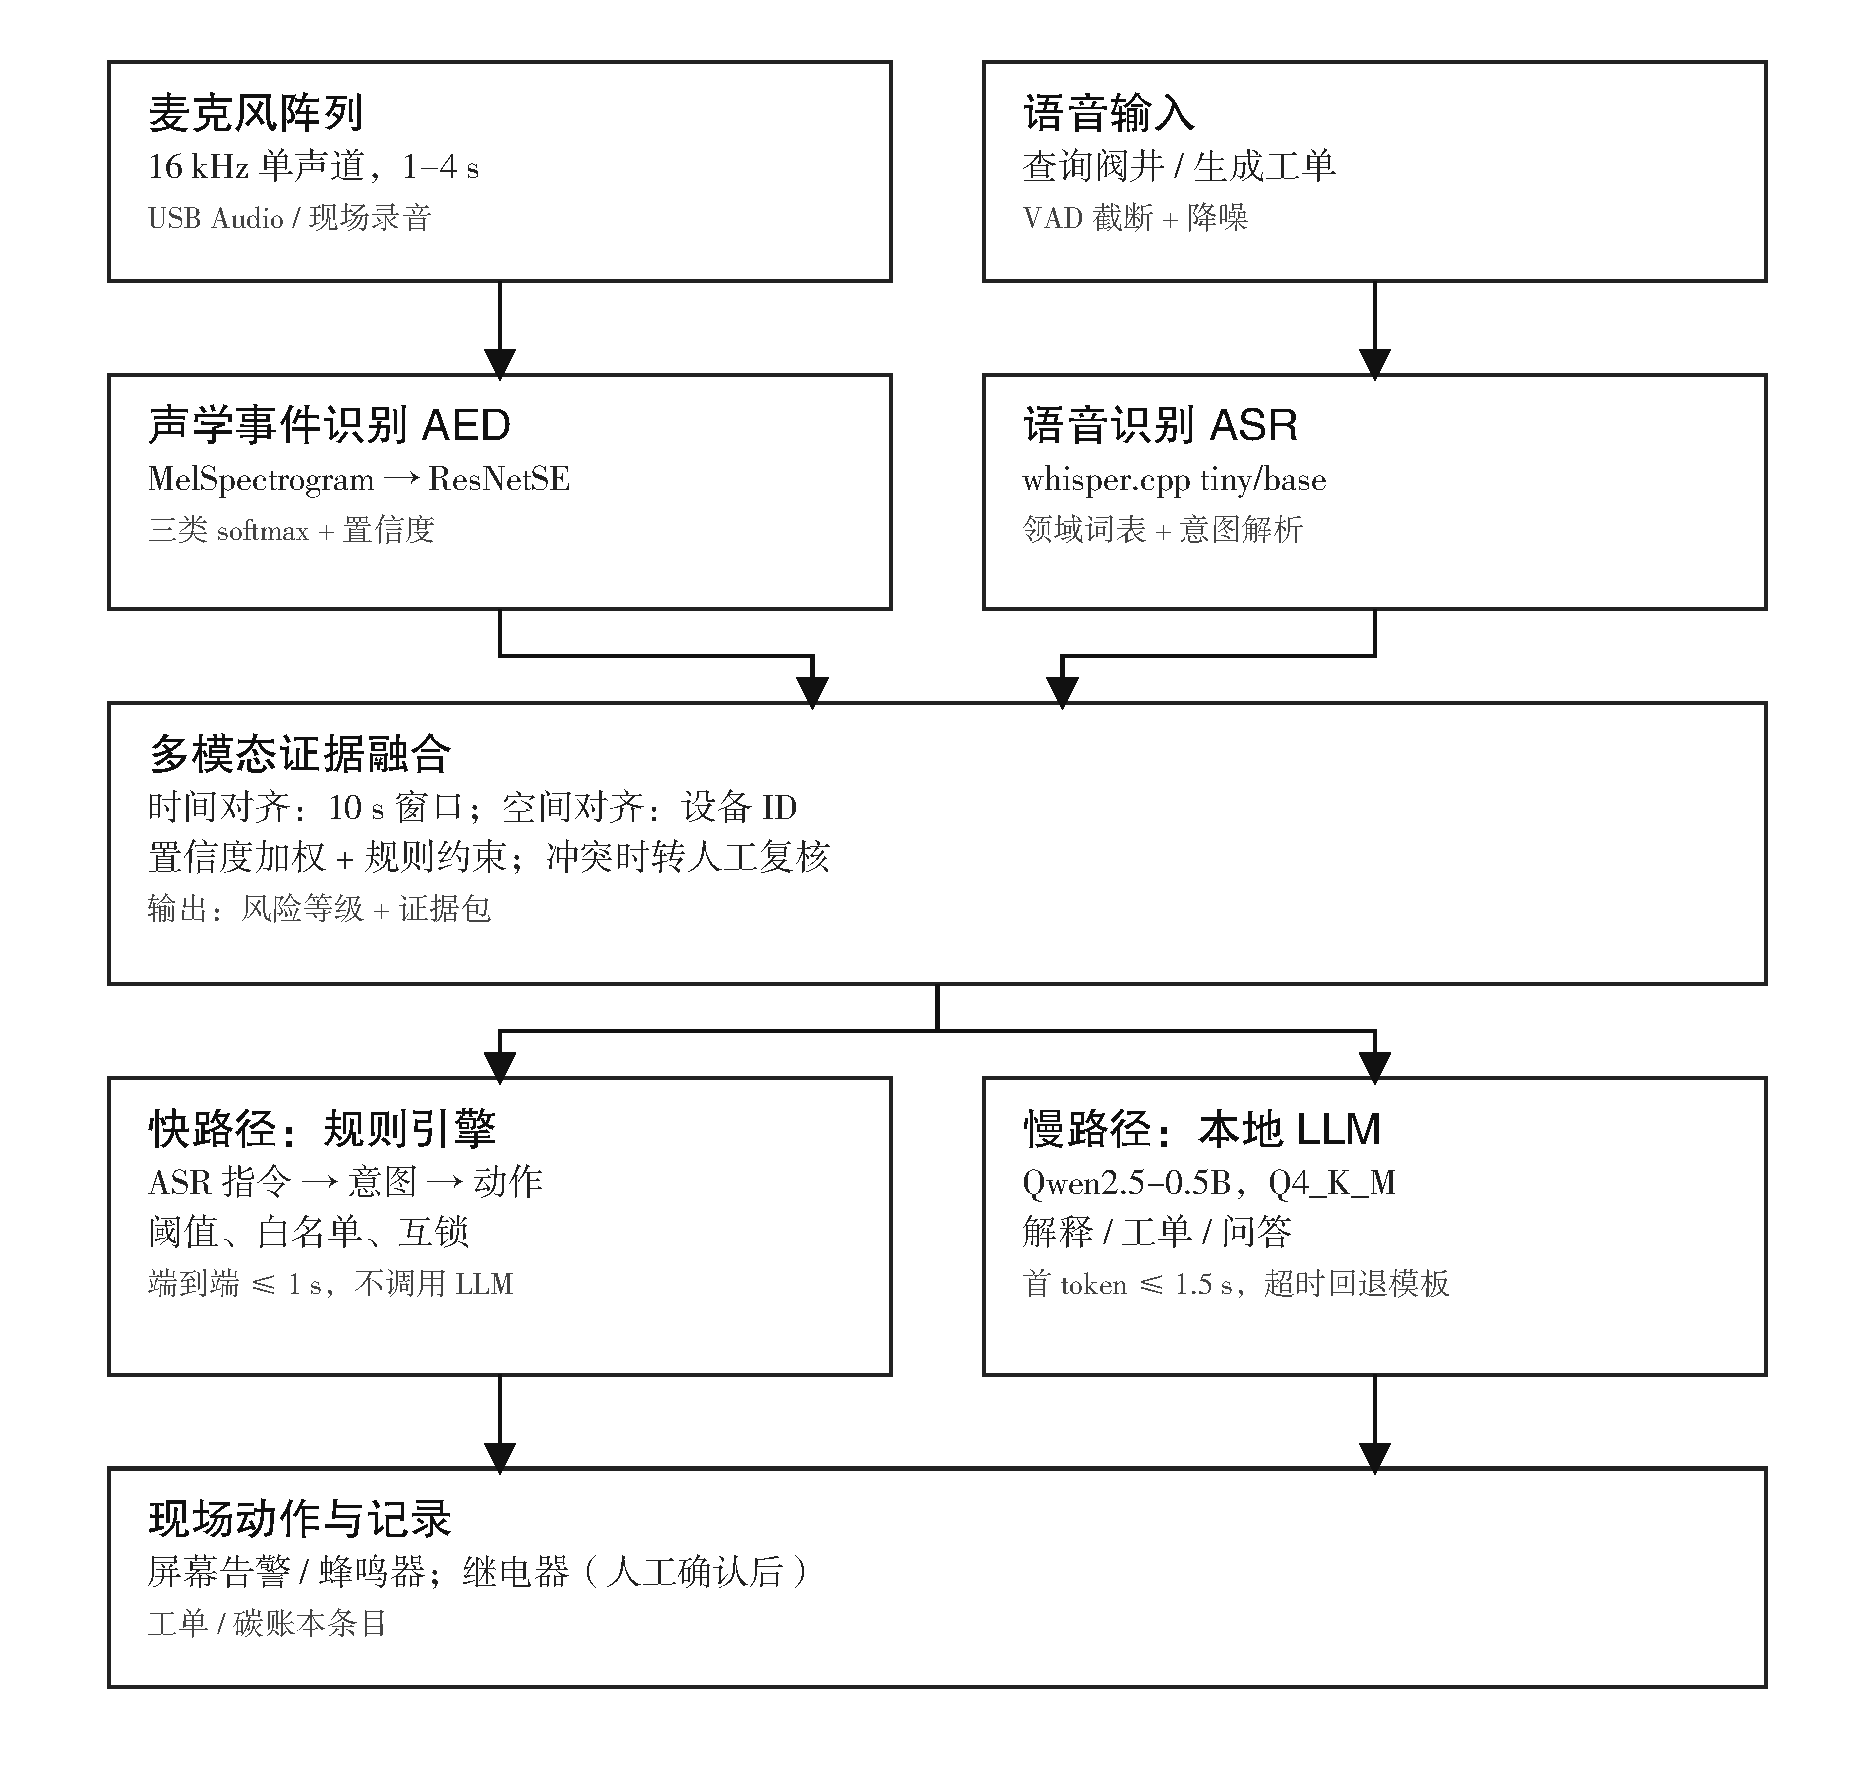
\includegraphics[width=0.90\linewidth]{figures/fig2_pipeline.pdf}
  \caption{快慢双路径多模态推理流水线}
  \label{fig:pipeline}
\end{figure}

快路径的时延预算为：音频解码与重采样 50 ms、Mel 特征 30 ms、ResNetSE 80--150 ms、规则/意图 20 ms、屏幕/继电器 20 ms，合计不超过 1 s。LLM 不在快路径上，首 token 目标为 1.5 s，完整工单目标为 8 s；超时自动回退模板。ASR 采用 VAD 截断、5 s 窗口、whisper.cpp \texttt{tiny}/\texttt{base} 量化模型与领域词表纠错\cite{whisper}；LLM 采用 Qwen2.5-0.5B 的 Q4\_K\_M 量化版本，2048 上下文\cite{qwen}。

\section{RISC-V 运行时适配}

把 PyTorch 模型放到 RISC-V 上，难点集中在运行时：PyPI 上的 torch 轮子主要面向 x86\_64 和 aarch64；torch、torchvision、torchaudio、numpy、av 必须来自同一套编译环境；librosa 依赖 numba JIT，而 numba 对 RISC-V 支持有限；libtorch、libgomp、libsleef、libstdc++ 的搜索路径需要显式配置；Bianbu 的 Python 版本、glibc、OpenMP 版本与通用 Ubuntu 镜像存在差异。

团队的基线是 Bianbu + 进迭时空 wheel 源 + torchaudio 音频前端 + Docker/CI。关键版本为 Python 3.12、PyTorch 2.8.0、torchvision 0.23.0、torchaudio 2.8.0、av 11.0.0、numba 0.62.1、llvmlite 0.43.0、Node.js 22。原项目使用 yeaudio 的 AudioSegment，RISC-V 上的稳定 wheel 供给有限；团队把音频前端替换为 torchaudio + soundfile，保持原有 API 不变。读取用 soundfile，绕开 torchaudio 新版本对 torchcodec 的依赖；重采样用 \path{torchaudio.transforms.Resample}，走 PyTorch 张量路径；音量归一化用 NumPy 的 RMS，与 librosa/scipy 解耦。

\begin{figure}[htbp]
  \centering
  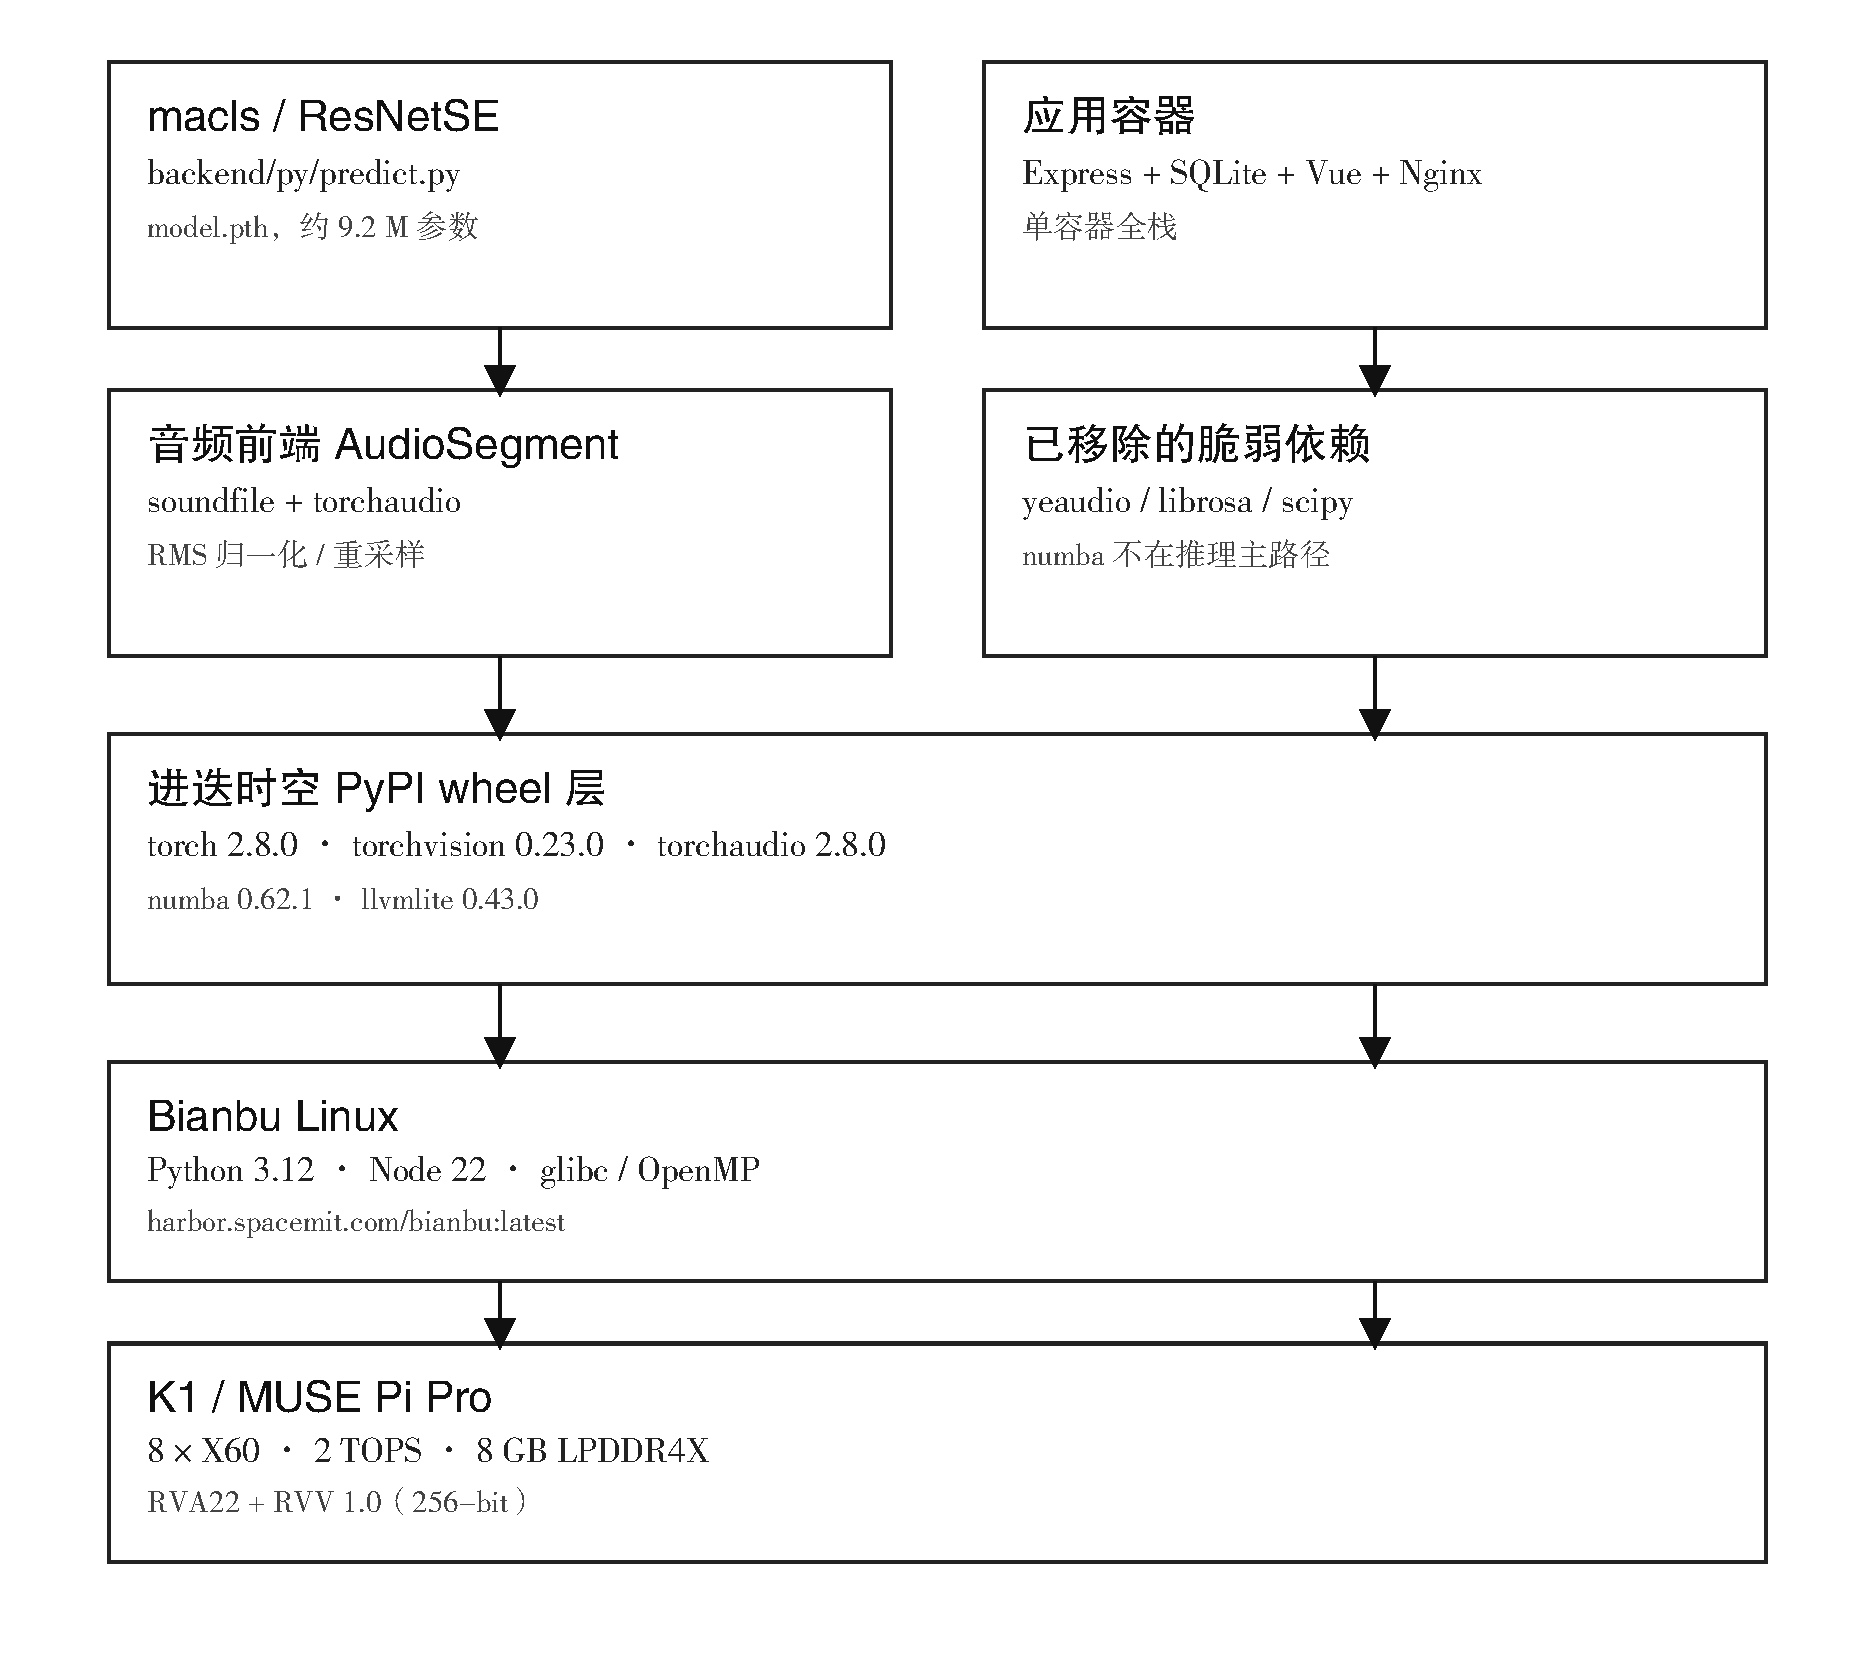
\includegraphics[width=0.92\linewidth]{figures/fig3_riscv_stack.pdf}
  \caption{RISC-V 深度学习运行时适配栈}
  \label{fig:stack}
\end{figure}

所有架构相关的二进制都从同一 SpacemiT wheel 源安装，不使用 \texttt{pip install torch} 的默认源。生产镜像的关键片段如下：

\begin{lstlisting}[language=bash,caption={RISC-V 运行时安装片段},label={lst:runtime}]
FROM harbor.spacemit.com/bianbu/bianbu:latest
ENV LD_LIBRARY_PATH="/usr/local/lib/python3.12/dist-packages/torch/lib:${LD_LIBRARY_PATH}"
RUN pip install --index-url https://git.spacemit.com/api/v4/projects/33/packages/pypi/simple \
    --trusted-host git.spacemit.com \
    torch==2.8.0 torchvision==0.23.0 torchaudio==2.8.0 \
    av==11.0.0 numba==0.62.1 llvmlite==0.43.0 --break-system-packages
RUN pip install ./whl/AudioClassification-Pytorch/ --break-system-packages
\end{lstlisting}

\section{优化策略与性能方案}

优化按“先消除结构性开销，再压缩计算量，最后做模型剪枝”的顺序推进。第一，把每次上传都冷启动 Python 进程改成常驻推理 worker，通过本地 HTTP 或 JSON Lines 复用已加载的模型，消除 36.8 MB 权重的重复加载和算子初始化。第二，对声学模型做动态或静态 INT8 量化，用 200 条校准样本检查量化前后精度，量化不达标时保留 FP32 快路径。第三，用 \texttt{taskset} 或 cgroup 给推理 worker 固定 4--6 个 X60 核，把 ASR、LLM、Web 服务分到不同 CPU 预算，减少迁移和争抢。第四，缓存 Mel 特征与模型 warmup 结果，减少首窗抖动。只有确认 INT8 与常驻 worker 仍不能满足时延预算，才按通道重要性剪枝 10--20\%，再用原模型蒸馏恢复精度；ResNetSE 的 shortcut 通道必须保留。

\begin{table}[htbp]
\centering
\small
\caption{优化项与验收口径}
\label{tab:optimization}
\begin{tabular}{p{3.6cm}p{6.4cm}p{4.4cm}}
\toprule
优化项 & 做法 & 验收口径 \\
\midrule
常驻 worker & 模型加载一次，JSON Lines/HTTP 复用 & 冷启动不再进入每次请求 \\
INT8 量化 & 200 条校准，保留 FP32 回退 & 精度下降不超过 2 个百分点 \\
线程与核隔离 & \texttt{taskset}/cgroup 固定 4--6 核 & p95 抖动收敛，Web 不阻塞推理 \\
缓存与预热 & 开机空推理，Mel 特征缓存 & 首窗时延可重复 \\
剪枝与蒸馏 & 通道重要性剪枝 10--20\% & 仅在量化后仍超预算时启用 \\
\bottomrule
\end{tabular}
\end{table}

\section{用户文档与部署说明}

系统采用“单容器全栈”部署：Nginx 提供前端静态文件和 \path{/api/} 反向代理，Node.js 后端监听 3000，Python 推理脚本由后端调用。生产镜像由 \texttt{Dockerfile.prod.riscv} 构建，基础镜像为 \path{harbor.spacemit.com/bianbu/bianbu:latest}，启动脚本 \texttt{start.sh} 同时拉起 Node 和 Nginx。

用户侧包含三类角色：管理员初始化系统、管理用户与查看全量记录；运维人员上传音频、查看风险等级与置信度、确认工单；现场人员通过触摸屏或语音查看告警、播放录音、确认复核。核心 API 包括 \path{/api/init-status}、\path{/api/init-admin}、\path{/api/login}、\path{/api/upload-audio}、\path{/api/audio-files}、\path{/api/audio-processing-status/:name} 和 \path{/api/test}；Swagger UI 在 \path{/api-docs}。

板端一键部署命令为：

\begin{lstlisting}[language=bash,caption={RISC-V 板端部署},label={lst:deploy}]
curl -sSL https://raw.githubusercontent.com/Lvshujun0918/AI_Water/refs/heads/main/install-riscv.sh | bash
# 浏览器访问板端 8080 端口，首次进入初始化管理员账户
\end{lstlisting}

部署检查包括：Bianbu 系统与 \texttt{riscv64} 架构、Docker/Compose 可用、\texttt{uploads/} 与 \texttt{db/} 目录 UID 1000 可写、镜像标签与提交 commit 一致、\path{/api/init-status} 返回正常、管理员默认密码已修改、上传 1--4 s WAV 后状态从“处理中”变为“完成”、断网后本地推理正常、日志与磁盘空间正常。

\section{测试报告}

本团队分别在以下环境进行测试：AMD64 开发机基线、K1 板端实测。AMD64 使用 Ryzen 7 PRO 8845HS、Python 3.11.2、PyTorch 2.8.0+cpu；输入为 4 s、16 kHz 单声道合成噪声，预热 10 次后连续运行 100 次。QEMU 使用 \texttt{riscv64/ubuntu:24.04}、Python 3.12.3、PyTorch 2.8.0+spacemit.0、torchaudio 2.8.0，CPU 设为 \texttt{rv64,v=true,vlen=256}，单线程运行 3 次。K1 板端实测采用进迭时空 K1 开发板进行测试。

\begin{table}[htbp]
\centering
\small
\caption{AMD64 模型基线}
\label{tab:amd64}
\begin{tabular}{p{3.4cm}p{3.6cm}p{6.2cm}}
\toprule
项目 & 实测值 & 说明 \\
\midrule
模型参数量 & 9,124,475 & ResNetSE，FP32 \\
权重文件 & 36,786,581 B & 约 35.1 MiB \\
模型加载 & 94.5 ms & 进程内加载，6 线程 \\
首窗推理 & 50.4 ms & 含读取、特征与一次前向 \\
热推理 p50/p95 & 30.3 / 34.9 ms & 100 次，6 线程 \\
线程扩展 p50 & 84.8 / 54.3 / 37.8 / 30.3 / 30.1 ms & 1 / 2 / 4 / 6 / 8 线程 \\
\bottomrule
\end{tabular}
\end{table}

\begin{table}[htbp]
\centering
\small
\caption{RISC-V 环境测试记录}
\label{tab:qemu}
\begin{tabular}{p{3.2cm}p{4.8cm}p{5.2cm}}
\toprule
项目 & 结果 & 说明 \\
\midrule
运行架构 & \texttt{riscv64} & \texttt{uname -m} \\
Python / PyTorch & 3.12.3 / 2.8.0+spacemit.0 & torchaudio 2.8.0 \\
模型加载 & 6.15 s & 单线程 \\
首窗推理 & 5.94 s & 4 s 合成音频 \\
热推理 p50/p95 & 1.33 / 2.50 s & 3 次，单线程 \\
\texttt{predict.py} CLI & 低风险，0.56815 & 端到端 30.25 s \\
\bottomrule
\end{tabular}
\end{table}


% =====================================================================
\chapter{开发计划}
\label{ch:plan}

\section{工作分解}

项目按“运行时—声学链路—多模态—系统集成—演示交付”推进，工作包与验收物如表\ref{tab:wbs}所示。

\begin{table}[htbp]
\centering
\small
\caption{开发工作分解}
\label{tab:wbs}
\begin{tabular}{p{1.4cm}p{3.6cm}p{6.0cm}p{3.0cm}}
\toprule
阶段 & 工作包 & 主要任务 & 验收物 \\
\midrule
P0 & 方案与运行时冻结 & 需求拆解、版本锁定、镜像骨架 & 方案书、Dockerfile \\
P1 & 声学链路 & 数据整理、训练、导出、上传推理 & 模型、predict.py、测试记录 \\
P2 & RISC-V 适配 & wheel 源、ABI、音频前端、QEMU 验证 & 镜像、启动脚本、模拟报告 \\
P3 & 多模态联调 & VAD、whisper.cpp、意图解析、LLM 工具调用 & 命令集、接口、联调记录 \\
P4 & 系统集成 & 权限、记录、碳账本、异常恢复 & Web 端、数据库、用户文档 \\
P5 & 板端测试 & K1 时延、功耗、稳定性、准确率 & 测试报告、原始 JSON \\
P6 & 演示交付 & 固定机位拍摄、讲解、字幕、提交 & 视频、提交清单 \\
\bottomrule
\end{tabular}
\end{table}

\section{风险与应对}

主要风险有四项。第一，K1 板端供应或系统版本不稳定，导致镜像无法复现；应对是保留 QEMU 验证路径，锁定 Bianbu 版本与 wheel 源，镜像按 commit 打标签。第二，ASR 在地下泵房噪声下识别率下降；应对是受限指令集、VAD、领域词表、置信度门槛和屏幕确认。第三，LLM 首 token 超时；应对是规则引擎快路径、模板回退、Q4 量化和 2048 上下文限制。第四，训练数据跨城市、跨季节泛化不足；应对是置信度阈值、人工复核和真实漏点样本回流。每个风险都对应一个可观测指标，避免只写“加强测试”。

% =====================================================================
\chapter{预期成果}
\label{ch:outcome}

\section{技术成果}

项目预期形成五项可交付成果：一台可在 K1 上离线运行的边缘检漏终端；一套包含声学识别、ASR、LLM 工具调用和碳账本的软件；一套可复现的 RISC-V 深度学习运行时与 Docker 镜像；一份包含优化策略、用户文档、部署说明和测试报告的技术文档；一段固定机位、带讲解的演示视频。源代码以 MIT 许可证开源，仓库地址见附录\ref{app:repo}。

\section{指标与验收口径}

表\ref{tab:targets}给出板端验收目标。

\begin{table}[htbp]
\centering
\small
\caption{板端验收目标}
\label{tab:targets}
\begin{tabular}{p{3.2cm}p{2.6cm}p{4.6cm}}
\toprule
指标 & 目标 & 当前证据 \\
\midrule
声学单窗 p95 & \(\leq300\) ms & AMD64 34.9 ms；QEMU 52.50 s  \\
语音指令端到端 & \(\leq1\) s & 设计预算合计 \(\leq1\) s  \\
ASR 3 s & \(\leq800\) ms & whisper.cpp base/int8 方案  \\
LLM 首 token & \(\leq1.5\) s & Qwen2.5-0.5B Q4\_K\_M  \\
冷启动 & \(\leq30\) s & 容器与常驻 worker 设计  \\
整机功耗 & \(\leq15\) W & 5 V/3 A 供电预算  \\
独立测试集准确率 & \(\geq90\%\) & 95.14\%  \\
\bottomrule
\end{tabular}
\end{table}

% =====================================================================
\chapter{应用价值与市场潜力}
\label{ch:value}

\section{水务价值}

漏损控制的第一收益是水费。以单个漏点 1.0 m\(^3\)/h、提前 27 天发现为例，节水量为 648 m\(^3\)；按供水综合电耗 0.3 kWh/m\(^3\) 计算，节电 194.4 kWh；按 0.5366 kgCO\(_2\)/kWh 的电网因子计算，减排 104.3 kgCO\(_2\)，扣除终端自身 23.5 kgCO\(_2\) 后净减排约 80.8 kgCO\(_2\)。这个数字不大，但已经为正；如果算上减少的水处理药剂、泵组磨损和爆管风险，实际收益更高。对供水企业而言，水费和电费的节省通常比碳收益更直接；碳账本把漏损控制纳入 ESG 披露和绿色融资的语言体系。

\section{市场与客户}

目标客户分为四类：城市供水企业的管网运维部门；二次供水与小区泵房运维单位；工业园区、园区水务和大型公共建筑；县域集中供水与农村供水工程。中国有数百个地级市和大量县域供水主体，管网末端监测、检漏和运维数字化是持续投入项。按“单城市 100--300 台终端、单台 0.8--1.5 万元”的静态假设测算，300 个城市的终端设备空间约为 2.4--13.5 亿元；若按设备价的 15\%--20\% 收取年度软件与运维服务费，年服务空间约为 0.36--2.7 亿元。该测算是量级说明，不是销售承诺，实际价格与数量以招标和试点结果为准。

\begin{table}[htbp]
\centering
\small
\caption{市场测算假设}
\label{tab:market}
\begin{tabular}{p{4.2cm}p{5.6cm}p{4.0cm}}
\toprule
变量 & 假设 & 说明 \\
\midrule
覆盖城市 & 300 个 & 地级市与重点县域 \\
单城市终端 & 100--300 台 & 按管网规模和重点阀井 \\
单台价格 & 0.8--1.5 万元 & 含终端、传感器与部署 \\
设备空间 & 2.4--13.5 亿元 & 静态测算 \\
年服务费 & 设备价的 15\%--20\% & 软件、算法与运维 \\
\bottomrule
\end{tabular}
\end{table}

\section{商业模式与推广路径}

商业模式采用“终端销售 + 软件授权 + 年度运维服务”的组合。第一阶段与供水企业做 1--2 个阀井/泵房的试点，按效果付费或联合课题验收；第二阶段把试点扩展到一个区的管网，形成标准部署包和运维 SOP；第三阶段通过水务集团、设计院和系统集成商复制到更多城市。终端的离线能力降低了网络改造门槛，碳账本则为水务企业的 ESG 报告和绿色金融提供可审计数据。

\section{竞争差异}

与人工听音相比，终端把“到现场听”变成“持续在线听”，把响应时间从小时级压缩到分钟级；与单纯声学记录仪相比，终端增加了 ASR、LLM 和碳账本，形成“发现—解释—工单—核算”的闭环；与云端方案相比，终端在断网阀井仍能工作，音频不出本地，隐私与带宽压力更小；与通用边缘盒子相比，团队把 RISC-V wheel 源、ABI、音频前端和 CI 固定下来，交付的是可复现的运行时，而不是一次性的演示镜像。

% =====================================================================
\section{结语}
\label{sec:conclusion}

城市供水管网漏损是一个同时牵动水、电、碳三个账本的问题，也天然适合边缘智能：数据在本地产生，决策要在本地完成，网络和云端只能是补充。本方案以进迭时空 K1 为底座，把声学检漏、语音交互、本地 LLM 与碳账本放进一台可离线运行的终端，并把 RISC-V 深度学习环境做成可复现的工程基线。这套方案的价值在于它具有在真实阀井断网运行、在无 GPU 的 2 TOPS 板端稳定工作的潜力，体现了 RISC-V 在智慧水务中的绿色基础设施价值。

% =====================================================================
\appendix

\chapter{开源仓库与复现入口}
\label{app:repo}

项目源代码已发布至 GitHub，采用 MIT 许可证：

\begin{center}
\large\url{https://github.com/Lvshujun0918/AI_Water}
\end{center}

仓库包含 Vue 3 前端、Express/SQLite 后端、PyTorch 声学模型、RISC-V Dockerfile、构建脚本、测试脚本和技术文档。

\printbibliography[title=参考资料]

\end{document}
